\chapter{Magnetic Fields and Magnetized Turbulence}
\label{ch:magnetic}

\marginnote{
\textbf{Suggested background reading:}
\begin{itemize} 
\item \href{http://adsabs.harvard.edu/abs/2012ARA\%26A..50...29C}{Crutcher, R.~M. 2012, ARA\&A, 50, 29} \nocite{crutcher12a}
\end{itemize}
\textbf{Suggested literature:}
\begin{itemize}
\item \href{http://adsabs.harvard.edu/abs/2008ApJ...684..380L}{Li, P.~S., McKee, C.~F., Klein, R.~I., \& Fisher, R.~T. 2008, ApJ, 684, 380} \nocite{li08a}
\end{itemize}
}

In our treatment of fluid flow and turbulence in Chapter \ref{ch:turbulence}, we concentrated on the hydrodynamic case. However, real star-forming clouds are highly magnetized. We therefore devote this chapter to the question of how magnetic fields change the nature of molecular cloud fluid flow.

\section{Observing Magnetic Fields}

\subsection{Zeeman Measurements}

We begin by reviewing the observational evidence for the existence and strength of magnetic fields in interstellar clouds. There are several methods that can be used to measure magnetic fields, but the most direct is the Zeeman effect. The Zeeman effect is a slight shift in the energy levels of an atom or molecule in the presence of a magnetic field. Ordinarily the energies of a level depend only the direction of the electron spin relative to its orbital angular momentum vector, not on the direction of the net angular momentum vector. However, in the presence of an external magnetic field, states with different orientations of the net angular momentum vector of the atom have slightly different energies due to the interaction of the electron magnetic moment with the external field. This causes levels that are normally degenerate to split apart slightly in energy. As a result, transitions into or out of these levels, which would normally produce a single spectral line, instead produce a series of separate lines at slightly different frequencies.

For the molecules with which we are concerned, the level is normally split into three sublevels -- one at slightly higher frequency than the unperturbed line, one at slightly lower frequency, and one at the same frequency. The strength of this splitting varies depending on the electronic configuration of the atom or molecule in question. For OH, for example, the splitting is $Z=0.98$ Hz/$\mu$G, where the parameter $Z$ is called the Zeeman sensitivity, and the shift is $\Delta \nu = BZ$, where $B$ is the magnetic field strength. Zeeman measurements target molecules where $Z$ is as large as possible, and these are generally molecules or atoms that have an unpaired electron in their outer shell. Examples include atomic hydrogen, OH, CN, CH, CCS, SO, and O$_2$.

\begin{marginfigure}
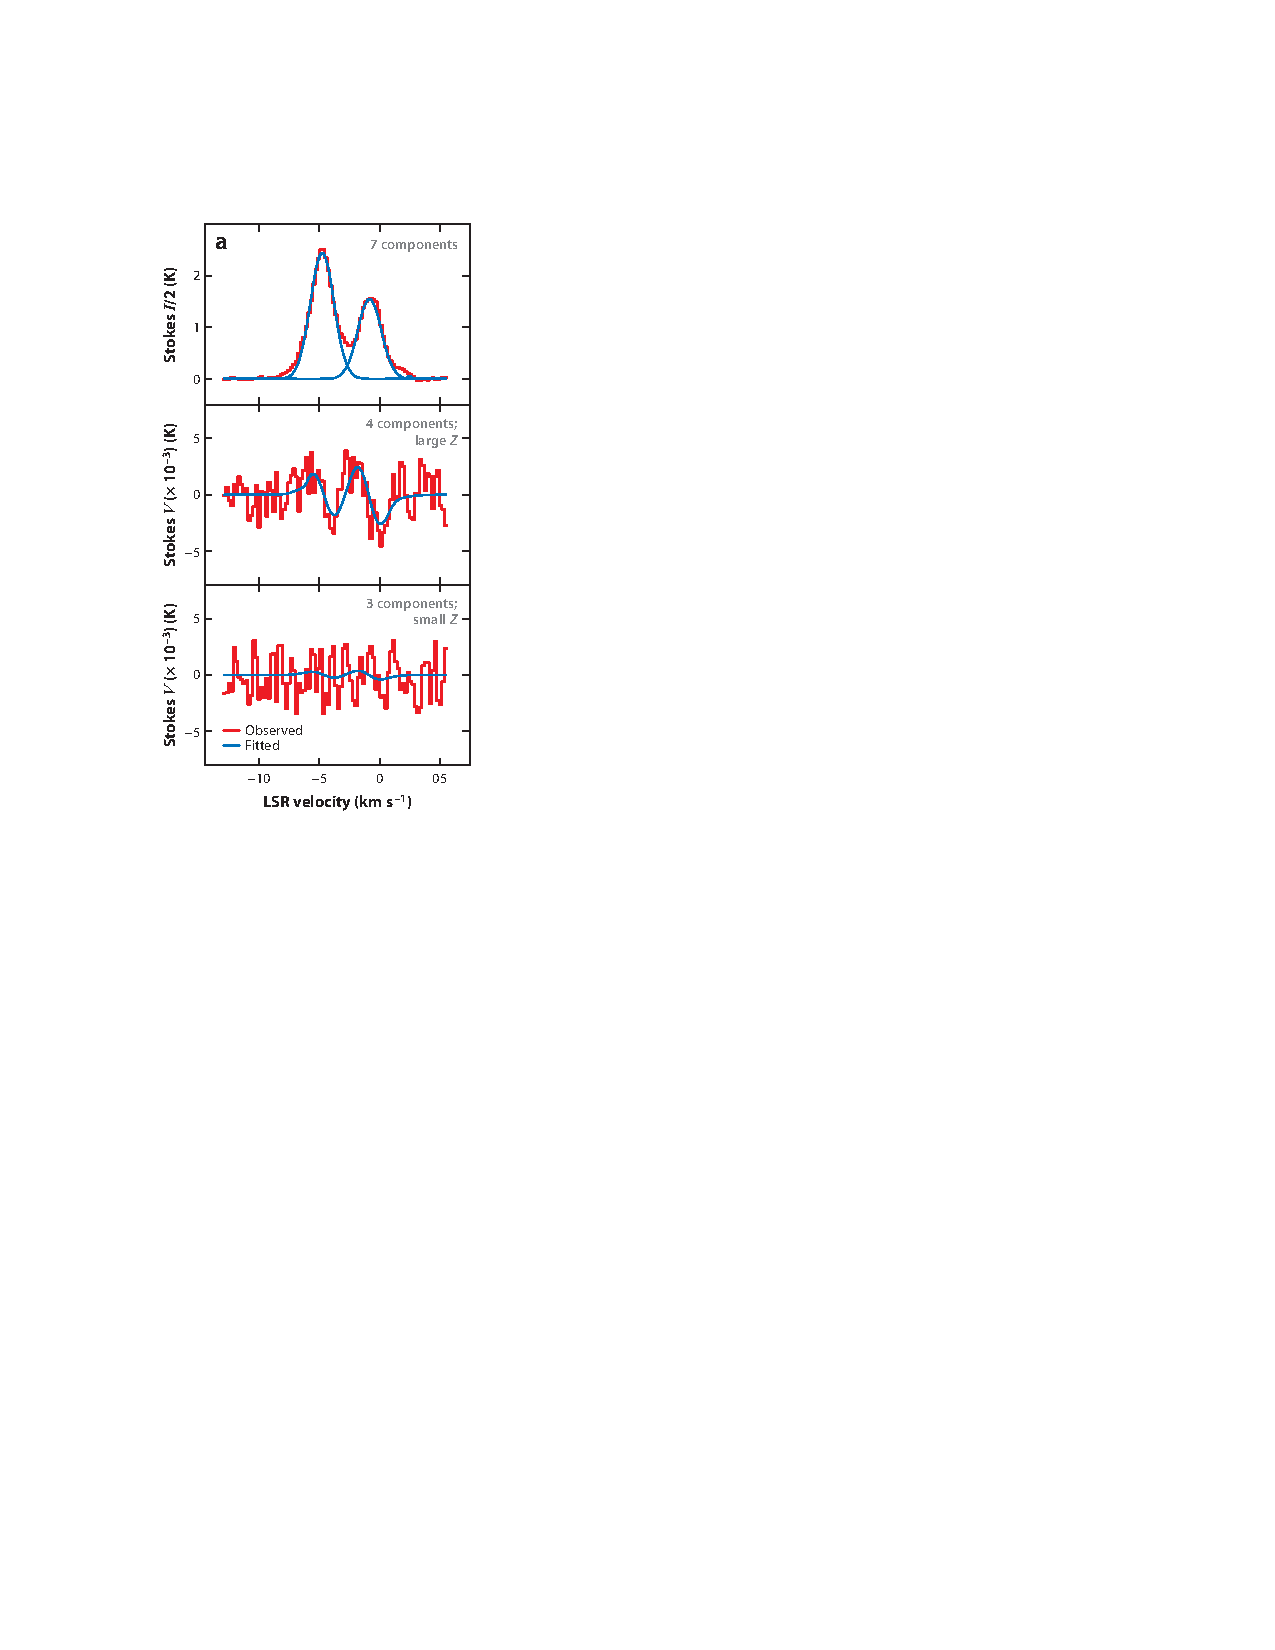
\includegraphics[width=\linewidth]{zeeman_crutcher}
\caption[Sample Zeeman detection of a magnetic field]{
\label{fig:zeeman}
Sample Zeeman detection of an interstellar magnetic field using the CN line in the region DR21(OH). The top panel shows the observed total intensity (Stokes $I$, red lines), which is well-fit by two different velocity components (blue lines). The CN molecule has 7 hyperfine components, of which 4 have a large Zeeman splitting and 3 have a small splitting. The middle panel shows the measured Stokes $V$ (circularly polarized emission) for the sum of the 4 strong splitting components, while the bottom panel shows the corresponding measurement for the 3 weak components. The smooth lines show the best fit, with the line of sight magnetic field as the fitting parameter. Credit: \citet{crutcher99b}, \copyright AAS. Reproduced with permission.
}
\end{marginfigure}
Zeeman splitting is not trivial to to measure due to Doppler broadening. To see why, consider the example of OH. The Doppler width of a line is $\sigma_{\nu} = \nu_0 (\sigma_v/c)$, where for the OH transition that is normally used for Zeeman measurements $\nu_0=1.667$ GHz. If the OH molecule has a velocity dispersion of order $0.1$ km s$^{-1}$, as expected even for the lowest observed velocity dispersions found on small scales in molecular clouds, then $(\sigma_v/c)\sim 10^{-6}$, so $\sigma_{\nu} \sim 1$ kHz. This means that, unless the field is considerably larger than $1000$ $\mu$G (1 mG), which it usually is not, the Zeeman splitting is smaller than the Doppler line width. Thus the split lines are highly blended, and cannot be seen directly in the spectrum.

However, there is a trick to avoid this problem: radiation from the different Zeeman sublevels has different polarization. If the magnetic field is along the direction of propagation of the radiation, emission from the higher frequency Zeeman sublevel is right circularly polarized, while radiation from the lower frequency level is left circularly polarized. The unperturbed level is unpolarized. Thus although one cannot see the line split if one looks at total intensity (as measured by the Stokes $I$ parameter), one can see that the different polarization components peak at slightly different frequencies, so that the circularly polarized spectrum (as measured by the Stokes $V$ parameter) looks different than the total intensity spectrum. One can deduce the magnetic field strength along the line of sight from the difference between the total and polarized signals. Figure \ref{fig:zeeman} shows a sample detection.

Applying this technique to line emission from molecular clouds indicates that they are threaded by magnetic fields whose strengths range from tens to thousands of $\mu$G, with higher density gas generally showing stronger fields. We can attempt to determine if this is dynamically important by a simple energy argument. For a low-density envelope of a GMC with $n\sim 100$ cm$^{-3}$ ($\rho \sim 10^{-22}$ g cm$^{-3}$), we might have $v$ of a few km s$^{-1}$, giving a kinetic energy density
\begin{equation}
e_K  = \frac{1}{2}\rho v^2 \sim 10^{-11}\mbox{ erg cm}^{-3}.
\end{equation}
For the magnetic field of $20$ $\mu$G, typical of molecular clouds on large scales, the energy density is
\begin{equation}
e_B = \frac{B^2}{8\pi} \sim 10^{-11} \mbox{ erg cm}^{-3}.
\end{equation}
Thus the magnetic energy density is comparable to the kinetic energy density, and is dynamically significant in the flow.

\subsection{The Chandrasekhar-Fermi Method}

While the Zeeman effect provides by far the most direct method of measuring magnetic field strengths, it is not the only method for making this measurement. Another commonly-used technique, which we will not discuss in any detail, is the Chandrasekhar-Fermi method \citep{chandrasekhar53a}. This method relies on the fact that interstellar dust grains are non-spherical, which has two important implications. First, a non-spherical grain acts like an antenna, in that it interacts differently with electromagnetic waves that are oriented parallel and perpendicular to its long axis. As a result, grains both absorb and emit light preferentially along their long axis. This would not matter if the orientations of grains in the interstellar medium were random. However, there is a second effect. Most grains are charged, and as a result they tend to become preferentially aligned with the local magnetic field. The combination of these two effects means that the dust in a particular region of the ISM characterized by a particular large scale magnetic field will produce a net linear polarization in both the light it emits and any light passing through it. The direction of the polarization then reveals the orientation of the magnetic field on the plane of the sky.

By itself this effect tells us nothing about the strength of the field -- in principle there should be some relationship between field strength and degree of dust polarization, but there are enough other compounding factors and uncertainties that we cannot with any confidence translate the observed degree of polarization into a field strength. However, if we have measurements of the field orientation as a function of position, then we can estimate the field strength from the morphology of the field. As we shall see below, the degree to which field lines are straight or bent is strongly correlated with the ratio of magnetic energy density to turbulent energy density, and so the degree of alignment becomes a diagnostic of this ratio. In fact, one can even attempt to make quantitative field strength estimates from this method, albeit with very large uncertainties.


\section{Equations and Characteristic Numbers for Magnetized Turbulence}

Now that we know that magnetic fields are present, we now turn to some basic theory for magnetized flow. To understand how magnetic fields affect the flows in molecular clouds, it is helpful to write down the fundamental evolution equation for the magnetic field in a plasma, known as the induction equation\footnote{One may find a derivation of this result in many sources. The notation we use here is taken from \citet{shu92a}.}
\begin{equation}
\label{eq:induction}
\frac{\partial \vecB}{\partial t} + \nabla \times (\vecB \times \vecv) = -\nabla \times (\eta \nabla \times \vecB)
\end{equation}
Here $\vecB$ is the magnetic field, $\vecv$ is the fluid velocity (understood to be the velocity of the ions, which carry all the mass, a distinction that will become important below), and $\eta$ is the electrical resistivity. If the resistivity is constant in space, we can use the fact that $\nabla \cdot \vecB=0$ to simplify this slightly to get
\begin{equation}
\label{eq:induction_eta}
\frac{\partial \vecB}{\partial t} + \nabla \times (\vecB \times \vecv) = \eta \nabla^2 \vecB.
\end{equation}
The last term here looks very much like the $\nu\nabla^2 \vecv$ term we had in the equation for conservation of momentum (equation \ref{eq:momentum}) to describe viscosity. That term described diffusion of momentum, while the one in this equation describes diffusion of the magnetic field.\footnote{We are simplifying quite a bit here. The real dissipation mechanism in molecular clouds is not simple resistivity, it is something more complex called ion-neutral drift, which is discussed in Section \ref{sec:non-ideal-mhd}. However, the qualitative analysis given in this section is unchanged by this complexity, and the algebra is significantly easier if we use a simple scalar resistivity.}

We can understand the implications of this equation using dimensional analysis much as we did for the momentum equation in Section \ref{ssec:reynolds_mach}. As we did there, we let $L$ be the characteristic size of the system and $V$ be the characteristic velocity, so $L/V$ is the characteristic timescale. Spatial derivatives have the scaling $1/L$, and time derivatives have the scaling $V/L$. We let $B$ be the characteristic magnetic field strength. Applying these scalings to equation (\ref{eq:induction_eta}), the various terms scale as
\begin{eqnarray}
\frac{BV}{L} + \frac{BV}{L} & \sim & \eta \frac{B}{L^2} \\
1 & \sim & \frac{\eta}{VL}
\end{eqnarray}
In analogy to the ordinary hydrodynamic Reynolds number, we define the magnetic Reynolds number by
\begin{equation}
\mbox{Rm} = \frac{LV}{\eta}.
\end{equation}
Magnetic diffusion is significant only if $\mathrm{Rm} \sim 1$ or smaller.

What is Rm for a typical molecular cloud? As in the hydrodynamic case, we can take $L$ to be a few tens of pc and $V$ to be a few km s$^{-1}$. The magnetic field $B$ is a few tens of $\mu$G. The electrical resistivity is a microphysical property of the plasma, which, for a weakly ionized plasma, depends on the ionization fraction in the gas and the ion-neutral collision rate. We will show in Section \ref{sec:non-ideal-mhd} that a typical value of the resistivity\footnote{Again keeping in mind that this is not a true resistivity, it is an order of magnitude effective resistivity associated with ion-neutral drift.} in molecular clouds is $\eta\sim 10^{22}-10^{23}$ cm$^2$ s$^{-1}$. If we consider a length scale $L\sim 10$ pc and a velocity scale $V\sim 3$ km s$^{-1}$, then $LV\sim 10^{25}$ cm$^2$ s$^{-1}$, then this implies that the Rm for molecular clouds is hundreds to thousands.

Again in analogy to hydrodynamics, this means that on large scales magnetic diffusion is unimportant for molecular clouds -- although it is important on smaller scales. The significance of a large value of Rm becomes clear if we write down the induction equation with $\eta=0$ exactly:
\begin{equation}
\frac{\partial \vecB}{\partial t} + \nabla \times (\vecB \times \vecv) = 0.
\end{equation}
To understand what this equation implies, it is useful consider the magnetic flux $\Phi$ threading some fluid element. We define this as
\begin{equation}
\Phi = \int_A  \vecB \cdot \nhat\, dA,
\end{equation}
where we integrate over some area $A$ that defines the fluid element. The time derivative of this is then
\begin{eqnarray}
\frac{d\Phi}{dt} & = & \int_A \frac{\partial\vecB}{\partial t}\cdot\nhat\, dA + \oint_{\partial A} \vecB\cdot \vecv \times d\mathbf{l} \\
& = & \int_A \frac{\partial\vecB}{\partial t}\cdot\nhat\, dA + \oint_{\partial A} \vecB\times \vecv \cdot d\mathbf{l}
\end{eqnarray}
where $\partial A$ is the boundary of $A$. Here the second term on the right comes from the fact that, if the fluid is moving at velocity $\vecv$, the area swept out by a vector $d\mathbf{l}$ per unit time is $\vecv\times d\mathbf{l}$, so the flux crossing this area is $\vecB\cdot \vecv\times d\mathbf{l}$. Then in the second step we used the fact that $\nabla\cdot \vecB = 0$ to exchange the dot and cross products.

If we now apply Stokes theorem again to the second term, we get
\begin{eqnarray}
\frac{d\Phi}{dt} 
& = & \int_A \frac{\partial\vecB}{\partial t}\cdot\nhat\, dA + \int_A \nabla\times (\vecB\times \vecv) \cdot \nhat\, dA \\
& = & \int_A \left[\frac{\partial\vecB}{\partial t} + \nabla\times (\vecB\times \vecv)\right]\cdot\nhat\,dA\\
& = & 0.
\end{eqnarray}
The meaning of this is that, when Rm is large, the magnetic flux through each fluid element is conserved. This is called flux-freezing, since we can envision it geometrically as saying that magnetic field lines are frozen into the fluid, and move along with it. Thus on large scales the magnetic field moves with the fluid. However, on smaller scales the magnetic Reynolds number is $\sim 1$, and the field lines are not tied to the gas. We will calculate this scale in Section \ref{sec:non-ideal-mhd}. Before doing so, however, it is helpful to calculate another important dimensionless number describing the MHD flows in molecular clouds.

The conservation of momentum equation including magnetic forces is
\begin{equation}
\frac{\partial}{\partial t}(\rho \mathbf{v}) = -\nabla \cdot(\rho \mathbf{v v}) - \nabla P + \rho \nu \nabla^2 \mathbf{v} + \frac{1}{4\pi} (\nabla\times\vecB)\times \vecB,
\end{equation}
and if we make order of magnitude estimates of the various terms in this, we have
\begin{eqnarray}
\frac{\rho V^2}{L} & \sim & -\frac{\rho V^2}{L} + \frac{\rho c_s^2}{L} + \frac{\rho \nu V}{L^2} + \frac{B^2}{L} \\
1 & \sim & 1 + \frac{c_s^2}{V^2} + \frac{\nu}{VL} + \frac{B^2}{\rho V^2}
\end{eqnarray}
The second and third terms on the right hand side we have already defined in terms of $\mathcal{M}= V/c_s$ and $\mathrm{Re} = LV/\nu$. We now define our fourth and final characteristic number,
\begin{equation}
\mathcal{M}_A \equiv \frac{V}{v_A},
\end{equation}
where
\begin{equation}
v_A = \frac{B}{\sqrt{4\pi \rho}}
\end{equation}
is the Alfv\'{e}n speed -- the speed of the wave that, in magnetohydrodynamics, plays a role somewhat analogous to the sound wave in hydrodynamics. In flows with $\mathcal{M}_A \gg 1$, which we refer to as super-Alfv\'{e}nic, the magnetic force term is unimportant, while in those with $\mathcal{M}_A \ll 1$, referred to as sub-Alfv\'{e}nic, it is dominant.

For characteristic molecular cloud numbers $n\sim 100$ cm$^{-3}$, $B$ of a few tens of $\mu$G, and $V$ of a few km s$^{-1}$, we see that $v_A$ is of order a few km s$^{-1}$, about the same as the velocity. Thus the flows in molecular clouds are highly supersonic ($\mathcal{M}\gg 1$), but only trans-Alfv\'{e}nic ($\mathcal{M}_A \sim 1$), and magnetic forces have a significant influence. These forces make it much easier for gas to flow along field lines than across them, and result in a pattern of turbulence that is highly anisotropic (Figure \ref{fig:alfvenmach}).

\begin{figure}
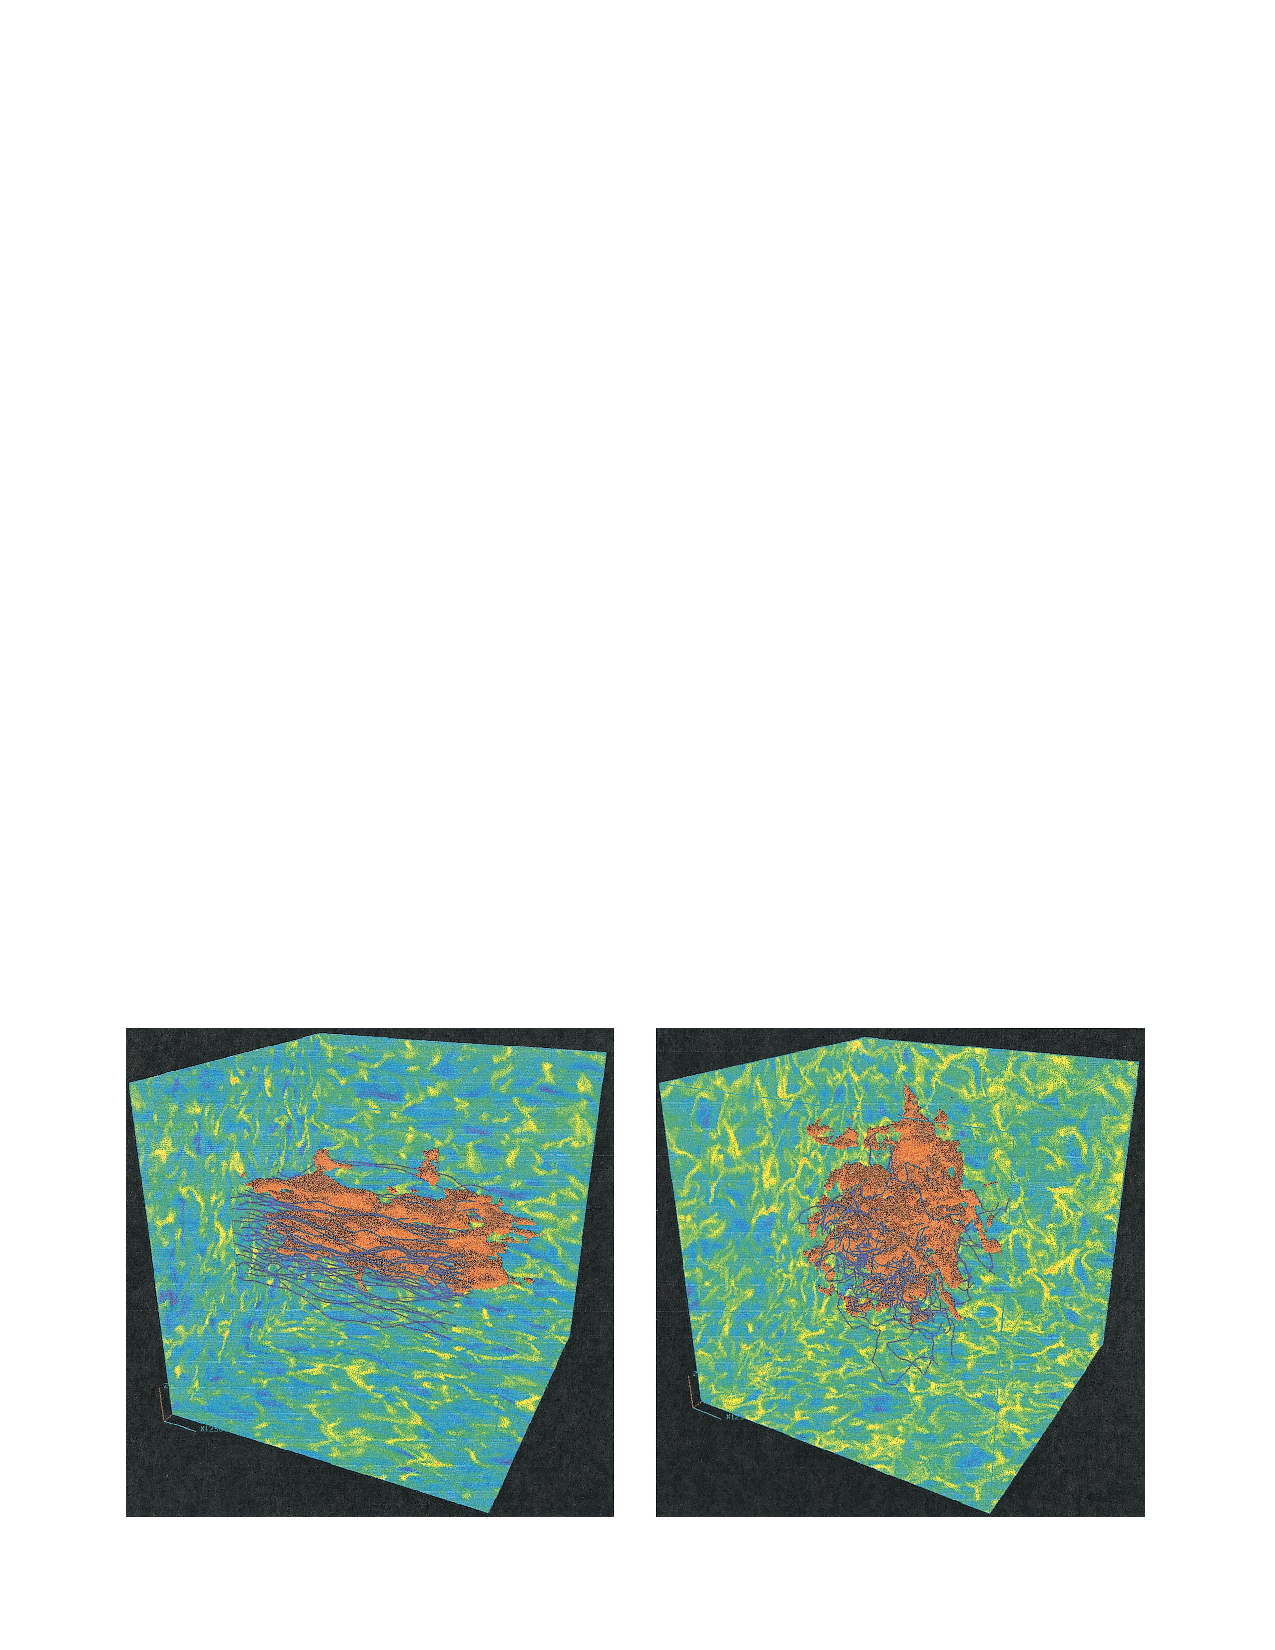
\includegraphics[width=\linewidth]{alfvenmach_stone98}
\caption[Comparison of simulations of Alfv\'{e}nic and sub-Alfv\'{e}nic turbulence]{
\label{fig:alfvenmach}
Simulations of sub-Alfv\'{e}nic (left) and Alfv\'{e}nic (right) turbulence. Colors on the cube surface are slices of the logarithm of density, blue lines are magnetic field lines, and red surfaces are isodensity surfaces for a passive contaminant added to the flow. Credit: \citet{stone98a}, \copyright\,AAS. Reproduced with permission.
}
\end{figure}

\section{Non-Ideal Magnetohydrodynamics}
\label{sec:non-ideal-mhd}

We have just shown that the magnetic Reynolds number is a critical parameter for magnetized turbulence, and that this depends on the resistivity $\eta$. In the final part of this Chapter we will discuss in a bit more detail the physical origins of resistivity and related effects.

\subsection{Ion-Neutral Drift}

Molecular clouds are not very good plasmas. Most of the gas in a molecular cloud is neutral, not ionized. The ion fraction may be $10^{-6}$ or lower. Since only ions and electrons can feel the Lorentz force directly, this means that fields only exert forces on most of the particles in a molecular cloud indirectly. The indirect mechanism is that the magnetic field exerts forces on the ions and electrons (and mostly ions matter for this purpose), and these then collide with the neutrals, transmitting the magnetic force.

If the collisional coupling is sufficiently strong, then the gas acts like a perfect plasma. However, when the ion fraction is very low, the coupling is imperfect, and ions and neutrals do not move at exactly the same speed. The field follows the ions, since the are much less resistive, and flux freeizing for them is a very good approximation, but the neutrals are able to drift across field lines. This slippage between ions and neutrals is called ion-neutral drift, or ambipolar diffusion.

To estimate how this process works, we need to think about the forces acting on both ions and neutrals. The ions feel a Lorentz force
\begin{equation}
\vecf_L = \frac{1}{4\pi} (\nabla \times \vecB) \times \vecB.
\end{equation}
The other force in play is the drag force due to ion-neutral collisions, which is
\begin{equation}
\vecf_d = \gamma\rho_n \rho_i (\vecv_i-\vecv_n),
\end{equation}
where the subscript $i$ and $n$ refer to ions and neutrals, respectively, and $\gamma$ is the drag coefficient, which can be computed from the microphysics of the plasma. In a very weakly ionized fluid, the neutrals and ions very quickly reach terminal velocity with respect to one another, so the drag force and the Lorentz force must balance. Equating our expressions and solving for $\vecv_d=\vecv_i-\vecv_n$, the drift velocity, we get
\begin{equation}
\vecv_d  = \frac{1}{4\pi\gamma\rho_n\rho_i}(\nabla\times\vecB)\times\vecB
\end{equation}

To figure out how this affects the fluid, we write down the equation of magnetic field evolution under the assumption that the field is perfectly frozen into the ions:
\begin{equation}
\frac{\partial \vecB}{\partial t} + \nabla\times(\vecB\times \vecv_i) = 0.
\end{equation}
To figure out how the field behaves with respect to the neutrals, which constitute most of the mass, we simply use our expression for the drift speed $\vecv_d$ to eliminate $\vecv_i$. With a little algebra, the result is
\begin{equation}
\frac{\partial \vecB}{\partial t} + \nabla\times(\vecB\times \vecv_n) = 
\nabla \times \left\{ \frac{\vecB}{4\pi\gamma\rho_n\rho_i}\times\left[\vecB\times(\nabla\times\vecB)\right]\right\}.
\end{equation}
Referring back to the induction equation (\ref{eq:induction}), we can see that the resistivity produced by ion-neutral drift is not a scalar, and that it is non-linear, in the sense that it depends on $\vecB$ itself.

However, our scaling analysis still applies. The magnitude of the resistivity produced by ion-neutral drift is
\begin{equation}
\eta_{\rm AD} = \frac{B^2}{4\pi\rho_i\rho_n\gamma}.
\end{equation}
Thus, the magnetic Reynolds number is
\begin{equation}
\mbox{Rm} = \frac{LV}{\eta_{\rm AD}} = \frac{4\pi L V \rho_i\rho_n\gamma}{B^2} \approx \frac{4\pi L V \rho^2 x\gamma}{B^2},
\end{equation}
where $x=n_i/n_n$ is the ion fraction, which we've assumed is $\ll 1$ in the last step. Ion-neutral drift will allow the magnetic field lines to drift through the fluid on length scales $L$ such that $\mbox{Rm}\lesssim 1$. Thus, we can define a characteristic length scale for ambipolar diffusion by
\begin{equation}
L_{\rm AD} = \frac{B^2}{4\pi\rho^2 x \gamma V}
\end{equation}

In order to evaluate this numerically, we must calculate two things from microphysics: the ion-neutral drag coefficient $\gamma$ and the ionization fraction $x$. For $\gamma$, the dominant effect at low speeds is that ions induce a dipole moment in nearby neutrals, which allows them to undergo a Coulomb interaction. This greatly enhances the cross-section relative to the geometric value. We will not go into details of that calculation, and will simply adopt the results: $\gamma\approx 9.2 \times 10^{13}$ cm$^3$ s$^{-1}$ g$^{-1}$ (\citealt{smith97a}; note that \citealt{shu92a} gives a value that is lower by a factor of $\sim 3$, based on an earlier calculation).

The remaining thing we need to know to compute the drag force is the ion density. In a molecular cloud the gas is almost all neutral, and the high opacity excludes most stellar ionizing radiation. The main source of ions is cosmic rays, which can penetrate the cloud, although nearby strong x-ray sources can also contribute if present. We have already discussed cosmic rays in the context of cloud heating and chemistry, and here too they play a central role. Calculating the ionization fraction requires balancing this against the recombination rate, which is a nasty problem. That is because recombination is dominated by different processes at different densities, and recombinations are usually catalyzed by dust grains rather than occurring in the gas phase. We will not go into the details of these calculations here, and will instead simply quote a rough fit to their results given by \citet{tielens05a},
\begin{equation}
n_i \approx 2\times 10^{-3}\mbox{ cm}^{-3} \left(\frac{n_{\rm H}}{10^4\mbox{ cm}^{-3}}\right)^{1/2} \left(\frac{\zeta}{10^{-16}\mbox{ s}^{-1}}\right)^{1/2},
\end{equation}
where $n_{\rm H}$ is the number density and $\zeta$ is the cosmic ray primary\footnote{I.e., counting only ionizations caused by direct cosmic ray hits, as opposed to ionizations caused when primary electrons go on to ionize additional atoms or molecules.} ionization rate. Thus at a density $n_{\rm H} \sim 100$ cm$^{-3}$, we expect $x\approx 10^{-6}$.

Plugging this into our formulae, along with our characteristic numbers $L$ of a few tens of pc, $V\sim$ a few km s$^{-1}$, and $B\sim 10$ $\mu$G, we find
\begin{eqnarray}
\mbox{Rm} & \approx & 50 \\
L_{\rm AD}& \sim & 0.5\mbox{ pc}.
\end{eqnarray}
If we put in numbers for $L$ and $V$ more appropriate for cores than entire GMCs, we get $L_{\rm AD} \sim 0.05$ pc. Thus we expect the gas to act like a fully ionized gas on scales larger than this, but to switch over to behaving hydrodynamically on small scales.

\subsection{Turbulent Reconnection}

A final non-ideal MHD effect that may be important in molecular clouds, though this is still quite uncertain, is turbulent reconnection. The general idea of reconnection is that, in regions of non-zero resistivity where oppositely directed field lines are brought into close contact, the field lines can break and the field geometry can relax to a lower energy configuration. This may allow the field to slip out of the matter, and it always involves a reduction in magnetic pressure and energy density. The released energy is transformed into heat.

The simplest model of reconnection, the Sweet-Parker model, considers two regions of oppositely-directed field that meet at a plane. On that plane, a large current must flow in order to maintain the oppositely-directed fields on either side of it. Within this sheet reconnection can occur. As with ion-neutral drift, we can define a characteristic Reynolds-like number for this process, in this case called the Lundqvist number:
\begin{equation}
\mathcal{R}_L = \frac{LV}{\eta},
\end{equation}
where here $\eta$ is the true microphysical resistivity, as opposed to the term describing ion-neutral diffusion.

The rate at which reconnection can occur in the Sweet-Parker model is dictated by geometry. Matter is brought into the thin reconnection region, it reconnects, and then it must exit so that new reconnecting matter can be brought in. Matter can only exit the layer at the Alfv\'{e}n speed, and since the cross-section of the reconnection layer is small, this sets severe limits on the rate at which reconnection can occur. It turns out that one can show that the maximum speed at which matter can be brought into the reconnection region is of order $\mathcal{R}_L^{1/2} v_A$.

To figure out this speed, we need to know the resistivity, which is related to the electrical conductivity $\sigma$ by
\begin{equation}
\eta = \frac{c^2}{4\pi \sigma}.
\end{equation}
We will not provide a full calculation of plasma conductivity here\footnote{Again, \citet{shu92a} is a good source for those who wish to see a rigorous derivation.}, but we can sketch the basic outlines of the argument. The conductivity of a plasma is the proportionality constant between the applied electric field and the resulting current,
\begin{equation}
J = \sigma E.
\end{equation}
In a plasma the current is carried by motions of the electrons, which move much faster than the ions due to their lower mass, and the current is simply the electron charge times the electron number density times the mean electron speed: $J = e n_e v_e$. To compute the mean electron speed, one balances the electric force against the drag force exerted by collisions with neutrals (which dominate in a weakly ionized plasma), in precisely the same way we derived the mean ion-neutral drift speed by balancing the drag force against the Lorentz force. Not surprisingly $v_e$ ends up being proportional to $E$, and inversely proportional to the number density of the dominant non-electron species (H$_2$ in molecular clouds) and the cross section of this species for electron collisions. The final result of this procedure is
\begin{equation}
\sigma = \frac{n_e e^2}{m_e n_{\rm H_2} \langle\sigma v\rangle_{e-\rm H_2}} \approx 10^{17} x\mbox{ s}^{-1},
\end{equation}
where $\langle\sigma v\rangle_{e-\rm H_2}\approx 10^{-9}$ cm$^3$ s$^{-1}$ is the mean cross-section times velocity for electron-ion collisions. Plugging this into the resistivity gives
\begin{equation}
\eta \approx \frac{10^3\mbox{ cm}^2\mbox{ s}^{-1}}{x}
\end{equation}
Plugging in our typical value $x\sim 10^{-6}$ gives $\eta\sim 10^{9}$ cm$^2$ s$^{-1}$, and using $L\sim 10$ pc and $V$ of a few km s$^{-1}$, typical molecular cloud numbers, this implies
\begin{equation}
\mathcal{R}_L \sim 10^{16}.
\end{equation}

Of course this makes the reconnection speed truly tiny, of order $10^{-8}$ of $v_A$. So why is reconnection at all interesting? Why is it worth considering? The answer turns on the word turbulent. It turns out that the Sweet-Parker model underpredicts the observed reconnection rate in laboratory experiments or observed in Solar flares and the Earth's magnetosphere. Indeed, if Sweet-Parker were right, there would be no such things as Solar flares.

We currently lack a good understanding of reconnection, but a rough idea is that, in a turbulent medium, reconnection sheets are can be much wider due to turbulent broadening, and that this in turn removes the geometric constraint that makes the reconnection velocity much smaller than the Alfv\'{e}n speed. Exactly how and when this is important in molecular clouds is a subject of very active debate in the literature.
